\chapter{Hardware}

Como ya se ha comentado previamente, el \textbf{hardware} es todo lo que forma parte del ordenador, que \textbf{puede ser tocado físicamente}. Dentro de un ordenador vamos a poder diferenciar distintos componentes que cumplirán una función distinta que detallaremos más adelante.

Es posible que ya conozcamos alguno de estos componentes, pero debemos conocer el origen y cómo surge la arquitectura de los ordenadores modernos.


\section{Arquitectura Von Neumann}

Las primeras computadoras electromecánicas eran diseñadas para un único propósito, estaban “diseñadas” para realizar una tarea. Un caso conocido puede ser \href{https://es.wikipedia.org/wiki/Bombe}{\textbf{Bombe}}, una máquina electromecánica capaz de descifrar los sistemas criptográficos nazis de Enigma. \movie{https://www.imdb.com/title/tt2084970/}{The Imitation Game}

Algunas se podían “reprogramar”, pero a base de recablear distintos componentes tras un estudio de lo que se quería realizar. Podía tomar hasta tres semanas preparar un programa de ENIAC y conseguir que funcionara.

El concepto de máquinas de computación universal y el uso de programa almacenado ya existía a nivel teórico desde mediados de la década de 1930 (escrito por \href{https://es.wikipedia.org/wiki/Alan_Turing}{Alan Turing}).

El matemático y físico \href{https://es.wikipedia.org/wiki/John_von_Neumann}{John von Neumann}, junto con otros compañeros, \textbf{describe en 1945 un diseño para una arquitectura de computadoras} en el que se describren los siguientes componentes que se interrelacionan entre sí a través del bus del sistema que actúa como canal de comunicación entre ellos:

\vspace{-10pt}
\begin{center}
    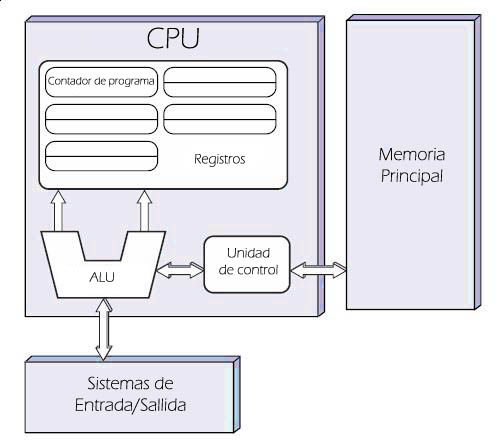
\includegraphics[width=0.5\linewidth]{vonneumann.jpg}
    \captionof{figure}{Arquitectura Von Neumann. Fuente: \href{https://es.wikipedia.org/wiki/Arquitectura_de_Von_Neumann}{wikipedia}}
\end{center}

\begin{itemize}
    \item \textbf{Unidad Central de Proceso} (\textbf{CPU}, por sus iniciales en inglés), que a su vez, contiene:
    \begin{itemize}
        \item \textbf{Unidad Aritmético Lógica} (\textbf{ALU} en inglés): Es un circuito digital que realiza operaciones aritméticas (suma, resta, multiplicaciones,...) y operaciones lógicas (AND, OR, X-OR,...) entre los valores de los argumentos (uno o dos).
        \item \textbf{Registros del procesador}: Memoria de alta velocidad y poca capacidad integrada en la CPU para almacenar datos utilizados durante la ejecución de un programa:
        \begin{itemize}
            \item Contador de programa
            \item Acumulador
            \item Registro de instrucciones
        \end{itemize}
        \item \textbf{Unidad de control}: Su función es buscar las instrucciones en la memoria principal, decodificarlas y ejecutarlas, empleando para ello la unidad de proceso.
    \end{itemize}
    \item La \textbf{memoria principal}: Sistema donde se almacenan las instrucciones y los datos del programa que se está ejecutando en ese instante, dividida en celdas que se identifican por medio de una única dirección.
    \item Los \textbf{sistemas de Entrada/Salida}: Realizan la transferencia de información entre periféricos de entrada y/o salida para extender las capacidades del equipo.
\end{itemize}


Hoy en día, los ordenadores han evolucionado, pero la arquitectura sigue siendo la misma, aunque más compleja.

\infobox{\textbf{Podemos ver una simulación de la Arquitectura Von Neumann \href{https://lab.xitrus.es/VonNeumann/}{aquí}}}


\section{Componentes básicos}


De manera general, podemos distinguir:

\begin{itemize}
    \item CPU / procesador
    \item Placa base
    \item Memoria
    \item Tarjetas gráficas
    \item Unidades de almacenamiento
    \item Fuente de alimentación
    \item Unidades de entrada
    \item Unidades de salida
    \item Unidades de entrada/salida
    \item Caja del ordenador
\end{itemize}



%
%\subsection{Procesador}
%
%\subsection{Placa base}
%
%\subsection{Memoria}
%
%
%
%
%\section{Arranque de un ordenador}
%
%\section{Periféricos}
%
%\section{Puertos de conexión}